\chapter{Theory}


\section{Wave Theory}

Simple Wave Theory

\section{Energy Spectra}

\subsection{Phillips Spectrum}
\subsection{Mobley Spectrum}
\subsection{SWAP}
\subsection{JONSWAP}


Energy Spectrum

$\int x(t) dt$

$k=\frac{\pi}{\mathbf y}$

\begin{equation}\label{eq:test} x = y \end{equation}

We can give an equation a label so that we can refer to it later.
\begin{equation}
\label{eq:ising}
E = -J \sum_{i=1}^N s_i s_{i+1} ,
\end{equation}
Equation~\eqref{eq:ising} expresses the energy of a configuration
of spins in the Ising model.

\section{The Rendering Pipeline}
The rendering pipeline constitutes the core of real-time graphics. It's task
consists in generating, or rendering, a two-dimensional output image given a
virtual camera, scene geometry, materials and
lightsources\cite{book:akenine-rtr}. As shown in Figure~\ref{fig:RAGR} the
rendering pipeline can be divided into three conceptual stages:
\begin{itemize}
 \item The \textit{application stage} holds all necessary information to break
down the scene geometry into smaller chunks which actually are passed on to the
geometry stage.
 \item The \textit{geometry stage} transforms the input geometry to a
two-dimensional output coordinate system.
 \item The \textit{rasterizer stage} fills the primitives output by the
geometry stage with color.
\end{itemize}

\begin{figure}
\begin{center}
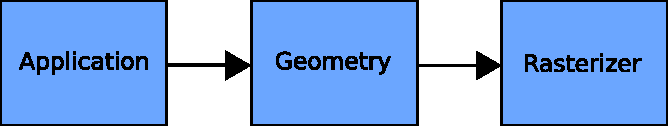
\includegraphics[scale=0.8]{Images/Rendering-Pipeline-AGR.pdf}
\caption{The three stages of the rendering pipeline.}
\label{fig:RAGR}
\end{center}
\end{figure}

\subsection{Application Stage}
The application stage implements the whole program logic. It's structure and
implementation is entirely dependent on the the task it should perform. One
such a task could be a simple triangle mesh visualisation, another, more
complex one, a complete 3D computer game. What these tasks have in common, is
that all of them require the application stage to provide the geometry stage
with appropriately prepared data for further processing.

Usually the application stage's main task is broken down into three subtasks:
\begin{itemize}
 \item Take \textit{user input}
 \item \textit{Update} the internal state
 \item \textit{Render} by feeding data to the next stage
\end{itemize}

A common task which resides in the application stage is \textit{collision
detection and response}: to detect if two objects collide and update their
internal state accordingly. Nowadays this is often done by a physics library,
such as \textit{NVIDIA PhysX}\cite{misc:ageia-physx} or \textit{Havok
Physics}\cite{misc:havok}.

In the case the application stage deals with large amounts of geometric
objects in a scene, it may prove necessary to reduce the amount of data which
is sent to the geometry stage. This is done by discarding objects invisible to
the viewer before they are actually handed over to the geometry stage,
effectively reducing the geometry stage's workload.

Whereas the geometry and rasterizer stages are to be found on the graphics
hardware, the application stage is typically executed in software on the CPU;
known exceptions are e.g. hardware accelerated physics and sound.

\subsection{Geometry Stage}
The geometry stage takes geometric primitives as input from the application
stage and processes them, so that the next stage, the rasterizer stage, may
calculate the final color for a pixel or fragment. In order to do that, the
geometric primitives have to be \textit{transformed} through several
\textit{coordinate systems}, eventually reaching the \textit{post-projection
space}. Transformations, such as rotation, translation, scaling and shearing,
usually are represented by matrices. For a three-dimensional space 4x4 matrices
are needed to be able to specify the aforementioned transformations. In
addition those transformations can be concatenated by multiplying the matrices
together, thereby reducing the arithmetic workload to compute multiple
transformations.

The \textit{model space} serves as starting point, as each model resides
therein, simply meaning that no transformation has been applied to the model
coordinates. By orienting and positioning such a model in the world, it gets
transformed to \textit{world space}. There may be more instances of the same
model in the world, possibly differing in orientation and position. The world
space itself is unique, all models are transformed with their respective model
transform and thereafter all are located in the world space. The next
coordinate system in the pipeline is the \textit{view space}, also known as
\textit{eye space}, which represents all objects or models in the world relative
to the camera position and camera viewing direction. The camera itself is able
to capture only a part of the world, depending on the camera's field of view
and viewing range. The volume the camera is actually able to see is called the
\textit{viewing volume}, better known as \textit{camera frustum}.
\FIXME{Coordinate frames and frustum illustration}

\begin{figure}
\begin{center}
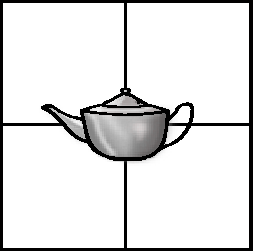
\includegraphics[scale=0.8]{Images/ModelSpace.pdf}
\caption{The Model Space.}
\label{fig:ModelSpace}
\end{center}
\end{figure}

parallel projection, parallel lines remain parallel
perspective projection parallel lines intersect each other at the vanishing
point

model coordinates
model matrix
world coordinates
view matrix
view coordinates
projection matrix
clip coordinates, cube
clipping
perspective division
normalized device coordinates, unit cube
viewport transformation
window coordinates
\begin{figure}
\begin{center}
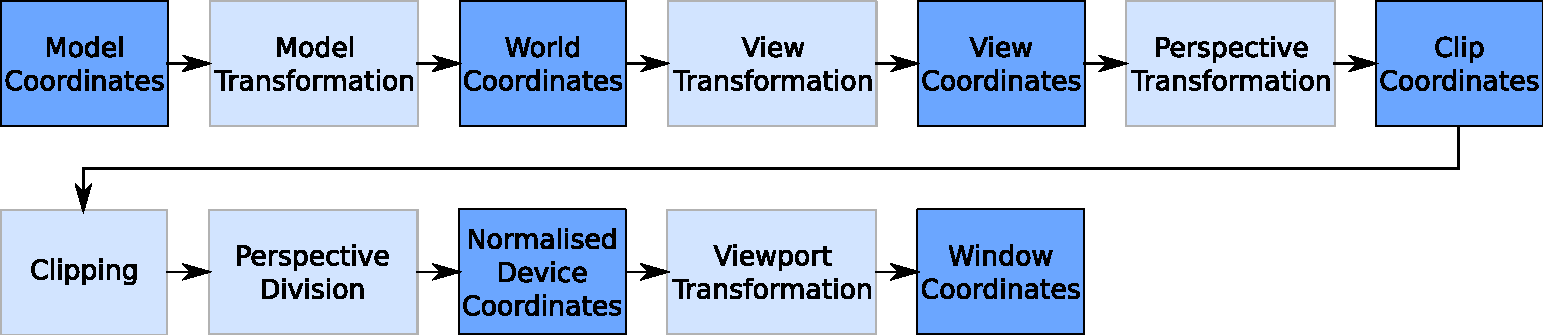
\includegraphics[scale=0.5]{Images/Geometry-Stage.pdf}
\caption{The Geometry stage.}
\label{fig:GeometryStage}
\end{center}
\end{figure}


\subsection{Rasterizer Stage}

triangle setup
scan conversion and interpolation
per fragment operations (texturing, ummadumshadern)
alpha test
depth test
stencil test
\begin{figure}
\begin{center}
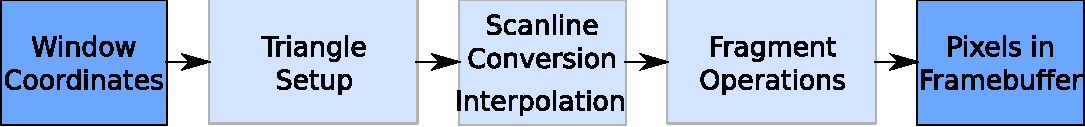
\includegraphics[scale=0.5]{Images/Rasterizer-Stage.pdf}
\caption{The Rasterizer stage.}
\label{fig:RasterizerStage}
\end{center}
\end{figure}

\section{The Projected Grid}

postprojection coordinates transformed to worldspace
grid on near and far plane, intersection with the y=0 plane
decouple projector from camera

\subsection{The Projector}
positioning
rotating
original is a hack, persistent grid mapping has a more stable approach
not optimal, because of "popping" at great distances
not so optimal distribution of the mesh resolution throughout worldspace
visual range issues
do some modifications to the mesh vertex distribution
reference to original paper from 2004 + persistent grid mapping

\section{Water optics}
BRAK

\section{Colour Management}

Explain color and gamma problem
linear vs nonlinear space

\subsection{gamma}
sRGB(gamma 2.2) support in hardware, convert from nonlinear space to linear
space do calculations on lighting and so on, back to srgb space
do tonemapping sRGB -> XYZ -> xyY -> modify Y -> XYZ -> sRGB

\subsection{device calibration}
short explanation of monitor calibration and so on
tools available


